\chapter{Implementation}
\paragraph{}The following is implementation and detailed description of different parts of the simulation

\section{Seesaw}
\paragraph{
The see saw is made using a rectangular box and a triangle
the Box is a object of Dynamic type whreas the triangle is of static type.
both are connected using a revolute joint \textbf{LINK}.which allows free rotation of the box about the vertex of the triangular base.
Initially a square block rests on the left arm of the seesaw.
the ball from top falls on right arm of the seesaw which projects the square block into the air.
}
\begin{figure}[H]
  \centering
    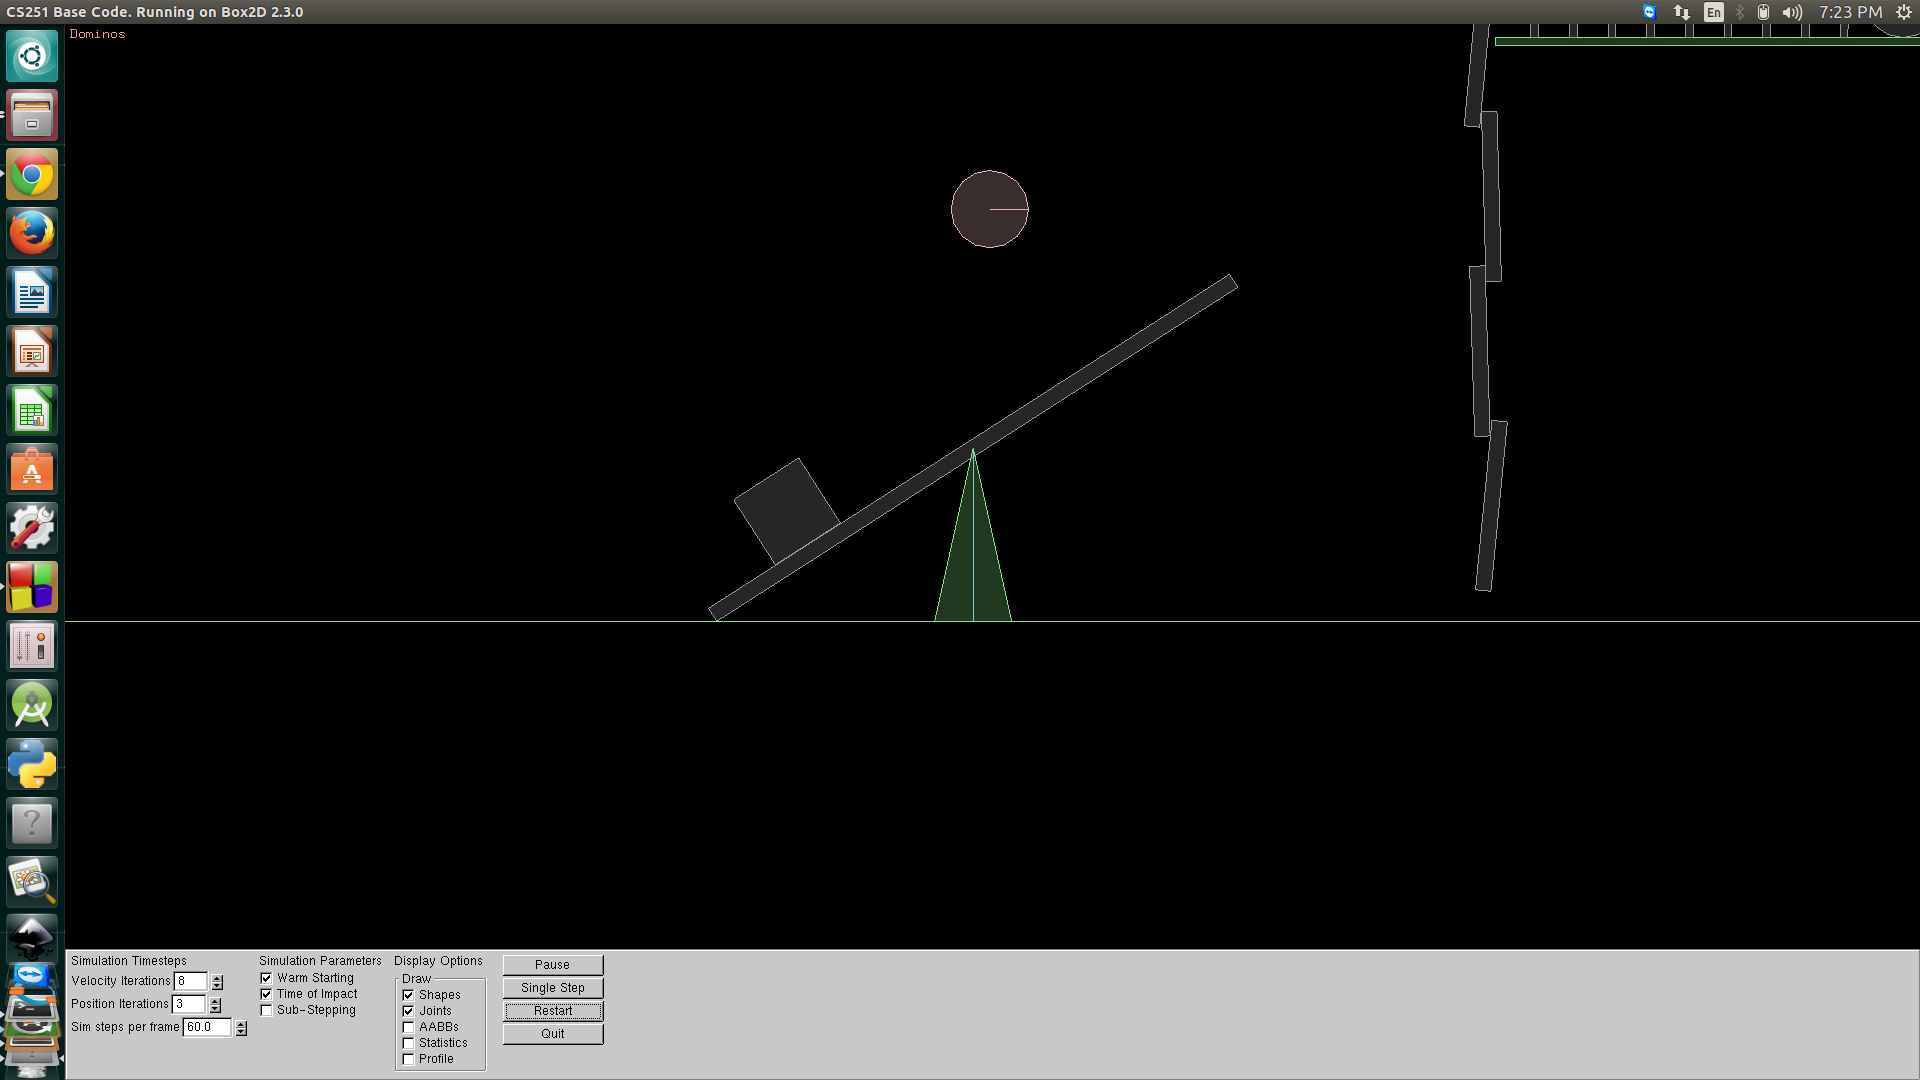
\includegraphics[scale=0.2]{project/images/pulley.png}
  \caption{\textbf{SEESAW}}
\end{figure}

\section{Pulley1}
\paragraph{
This pulley is made using an open box and a long rectangular box which are connected using the pulley joint\textbf{LINK},which makes one body move up when the other moves down and vice-versa.
Initially the pulley is balanced ie.,weights of open box and the long planc are balanced.
now the square block which flew from the left arm of the seesaw falls in the open box connected to the left arm of the pulley.
the pulley gets unbalancedand hence the open box starts going down and the plank on the right side starts to rise.
It then collides with a rotatable planc on which a ball is resting
}
\begin{figure}[H]
  \centering
    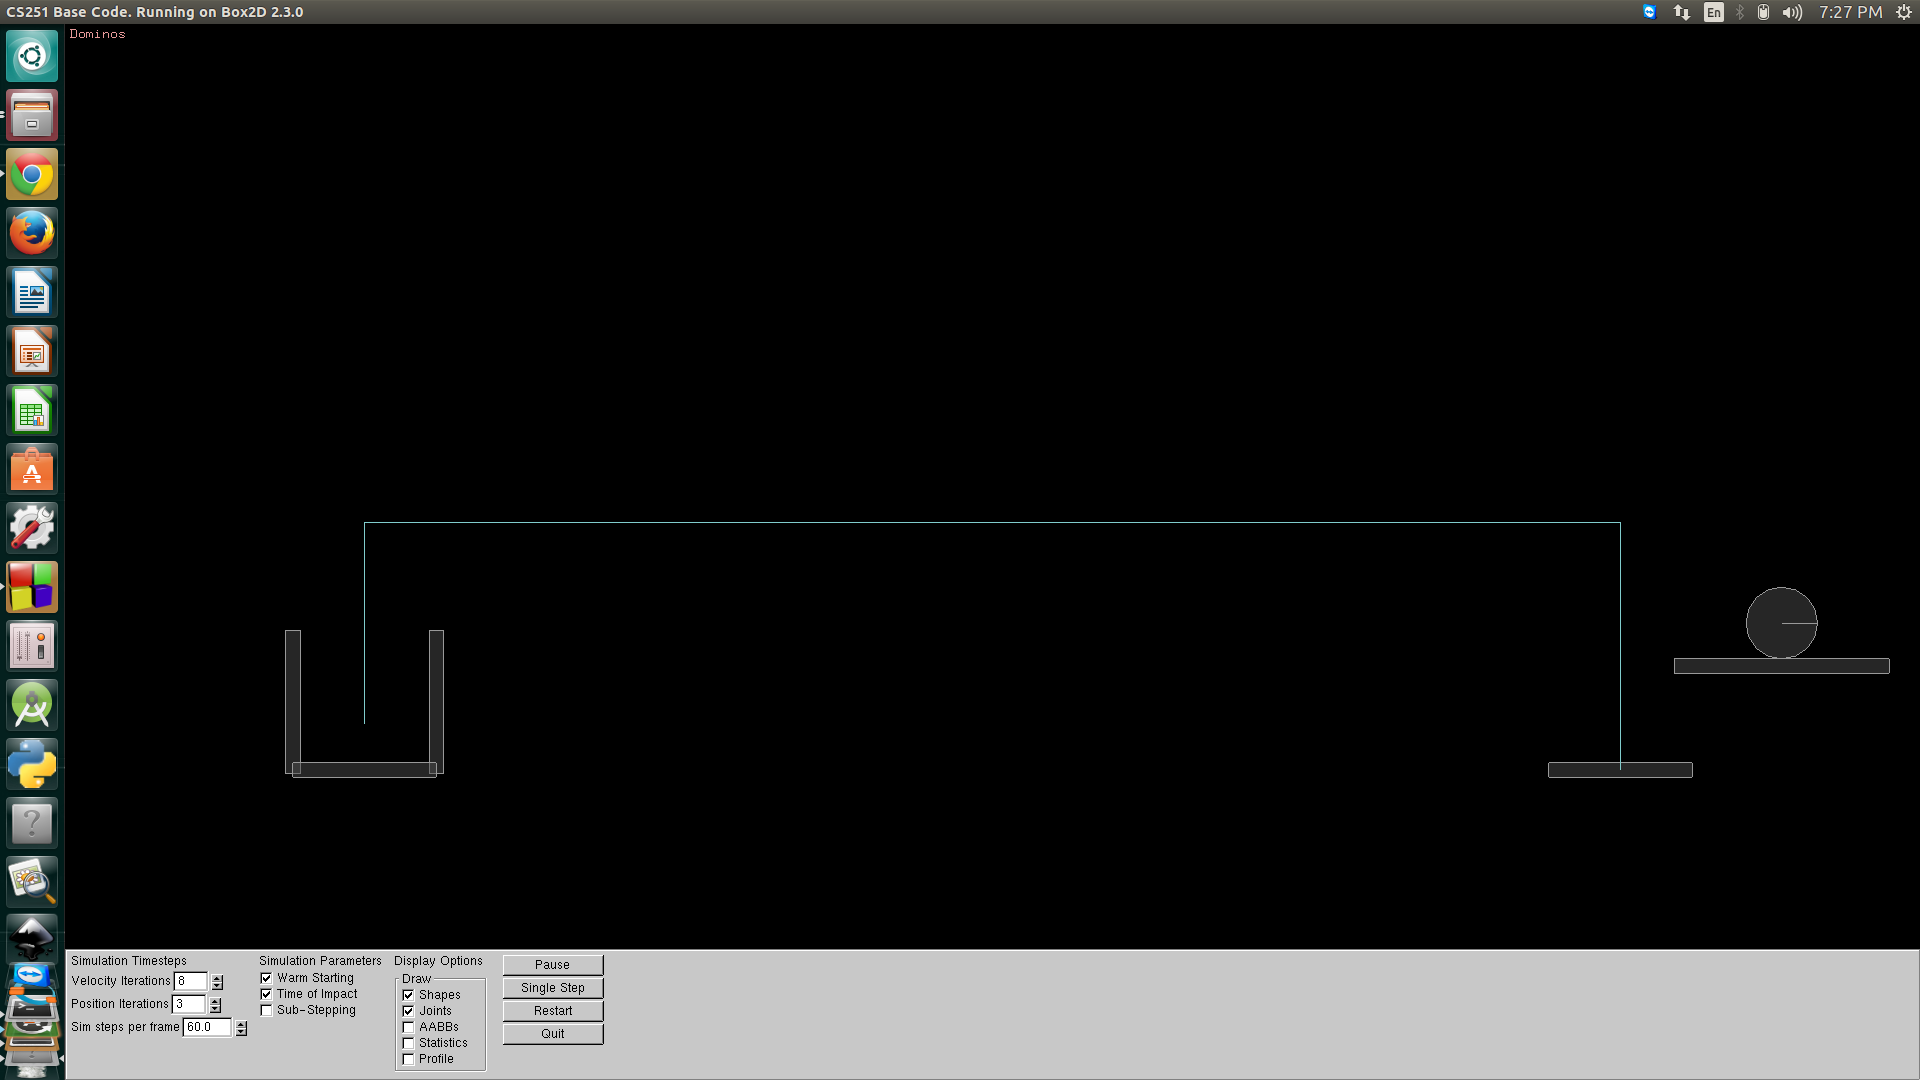
\includegraphics[scale=0.2]{project/images/pulley2.png}
  \caption{\textbf{PULLEY}}
\end{figure}


\section{the set of rotatable plancks}
\paragraph{
These are made using a rectangular block and a small static box used as the hinge at the ceter which are connected using the revolute joint\textbf{LINK},which makes the planck free to rotate about it's center.
Meanwhile the first ball which fell on the left arm of the seesaw falls of the seesaw and goes right and hits the lowest plank.
which triggers a series of collisions between the rotatable planks.
the top most plank now collides with the dominoes.
the dominoes now get triggered and the fall one by one and finally they collide with a ball which starts moving right.
}
\begin{figure}[H]
  \centering
    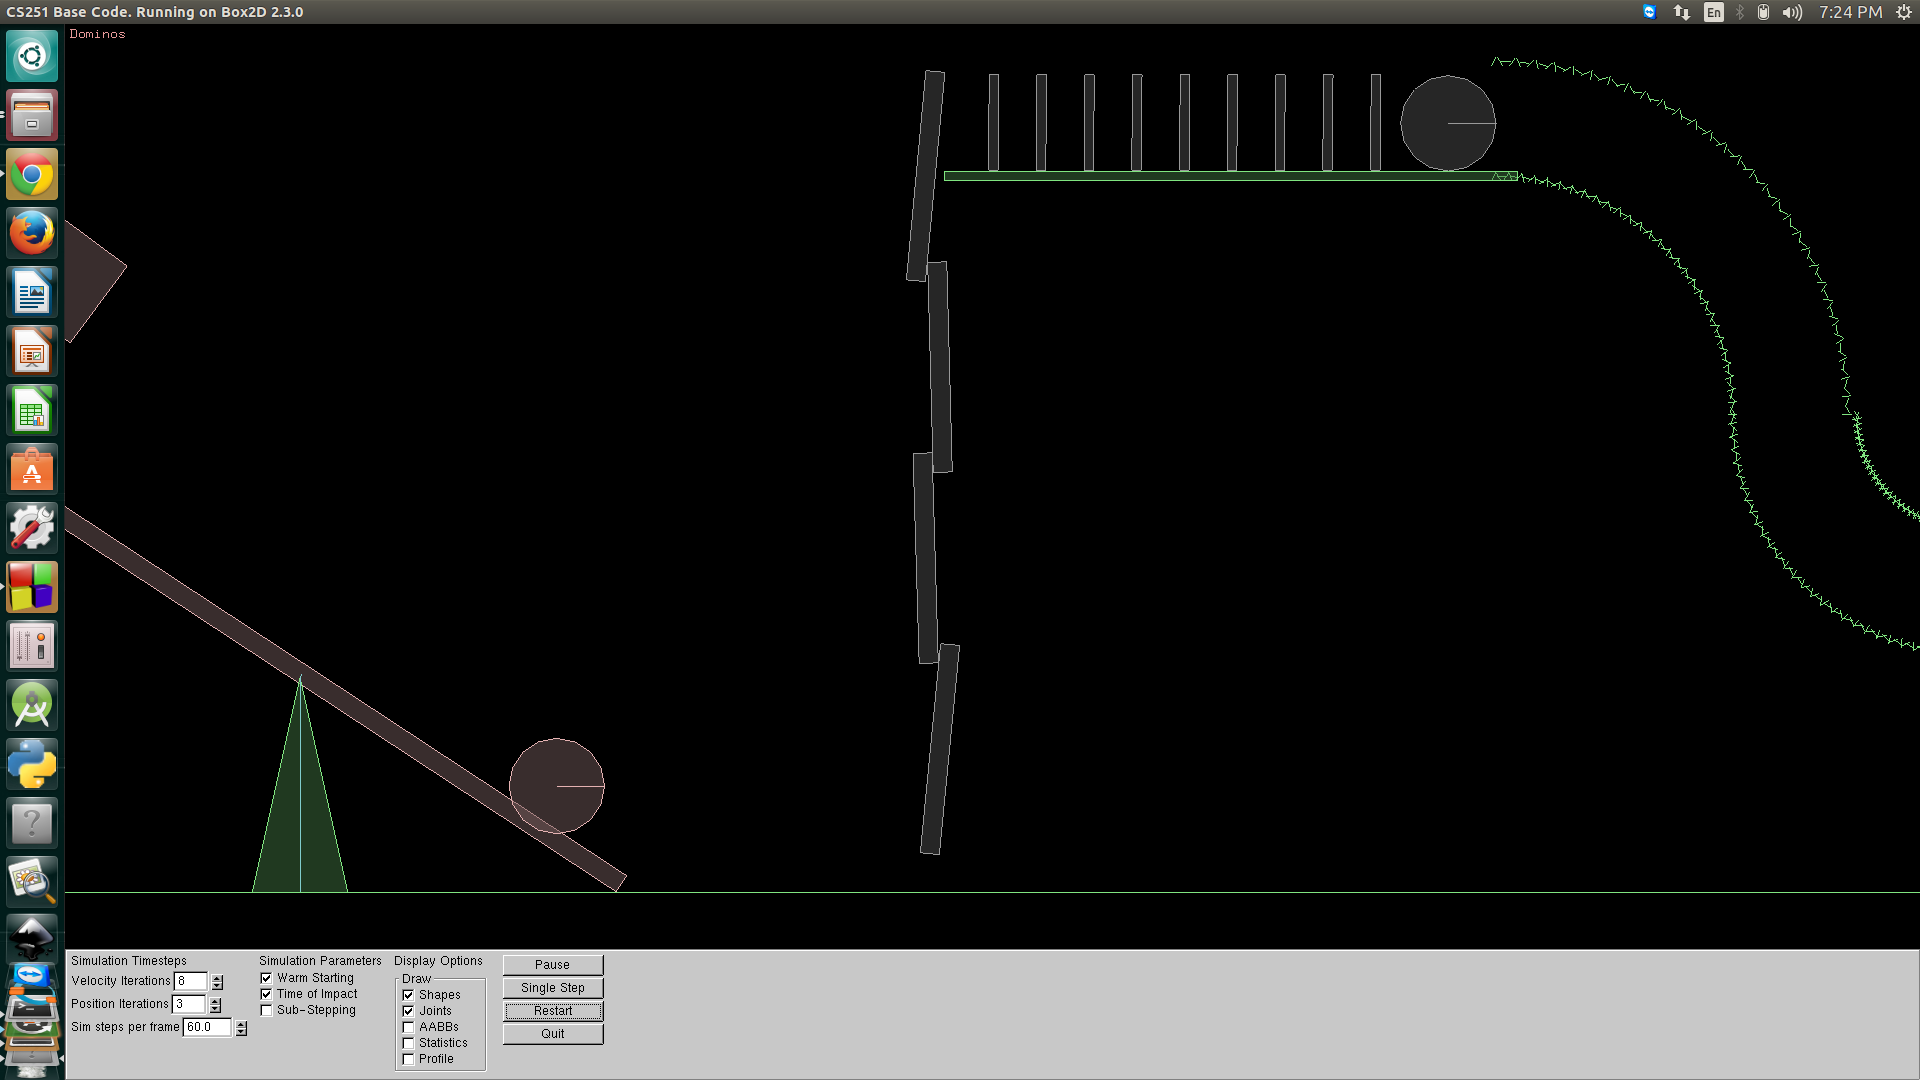
\includegraphics[scale=0.2]{project/images/plating.png}
  \caption{\textbf{ROTATABLE PLANES}}
\end{figure}

\section{the second set of rotatable plancks}
\paragraph{
These are made using a rectangular block and a small static box used as the hinge at the ceter which are connected using the revolute joint\textbf{LINK},which makes the planck free to rotate about it's center.
Meanwhile the floating  ball which                                moves up and hits the leftmost plank,which triggers a series of collisions between the rotatable planks each of which is supporting a ball.each plank rotates and triggers the next plank to rotate by colliding.now all the planks rotate and all the balls on them fall on the static ramp below them.
}
\begin{figure}[H]
  \centering
    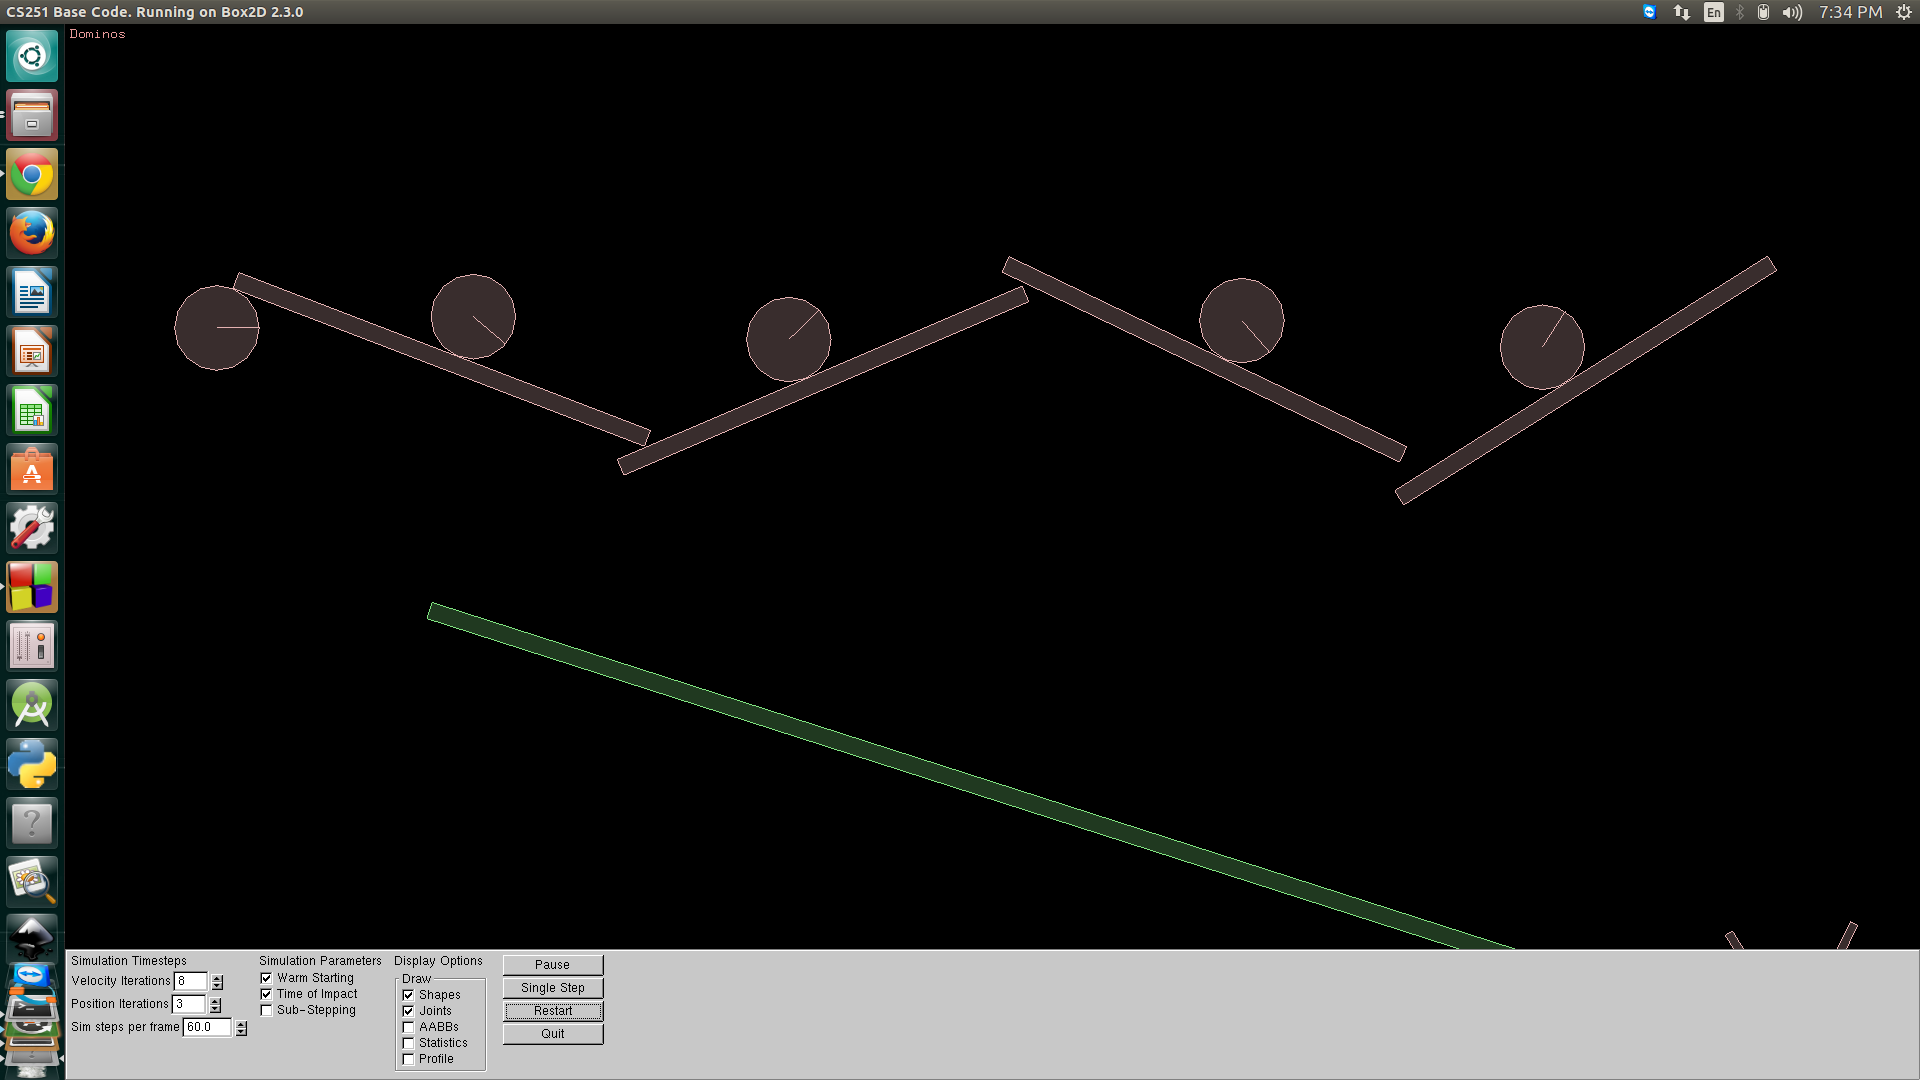
\includegraphics[scale=0.2]{project/images/revolvers.png}
  \caption{\textbf{SECOND SET OF ROTATING PLANES}}
\end{figure}

\section{The motor}
\paragraph{
These are made using 3 thin rectangular blocks and a small static box used as the hinge at the ceter which are connected using the revolute joint\textbf{LINK},which makes the plancs free to rotate about it's center.also the motor feature of the revolute joint is enabled so that it rotates at a particular speed.
Meanwhile the  balls come rolling on the ramp fall on the motor.
The motor sends the balls one by one into the open box of the second pulley.
}
\begin{figure}[H]
  \centering
    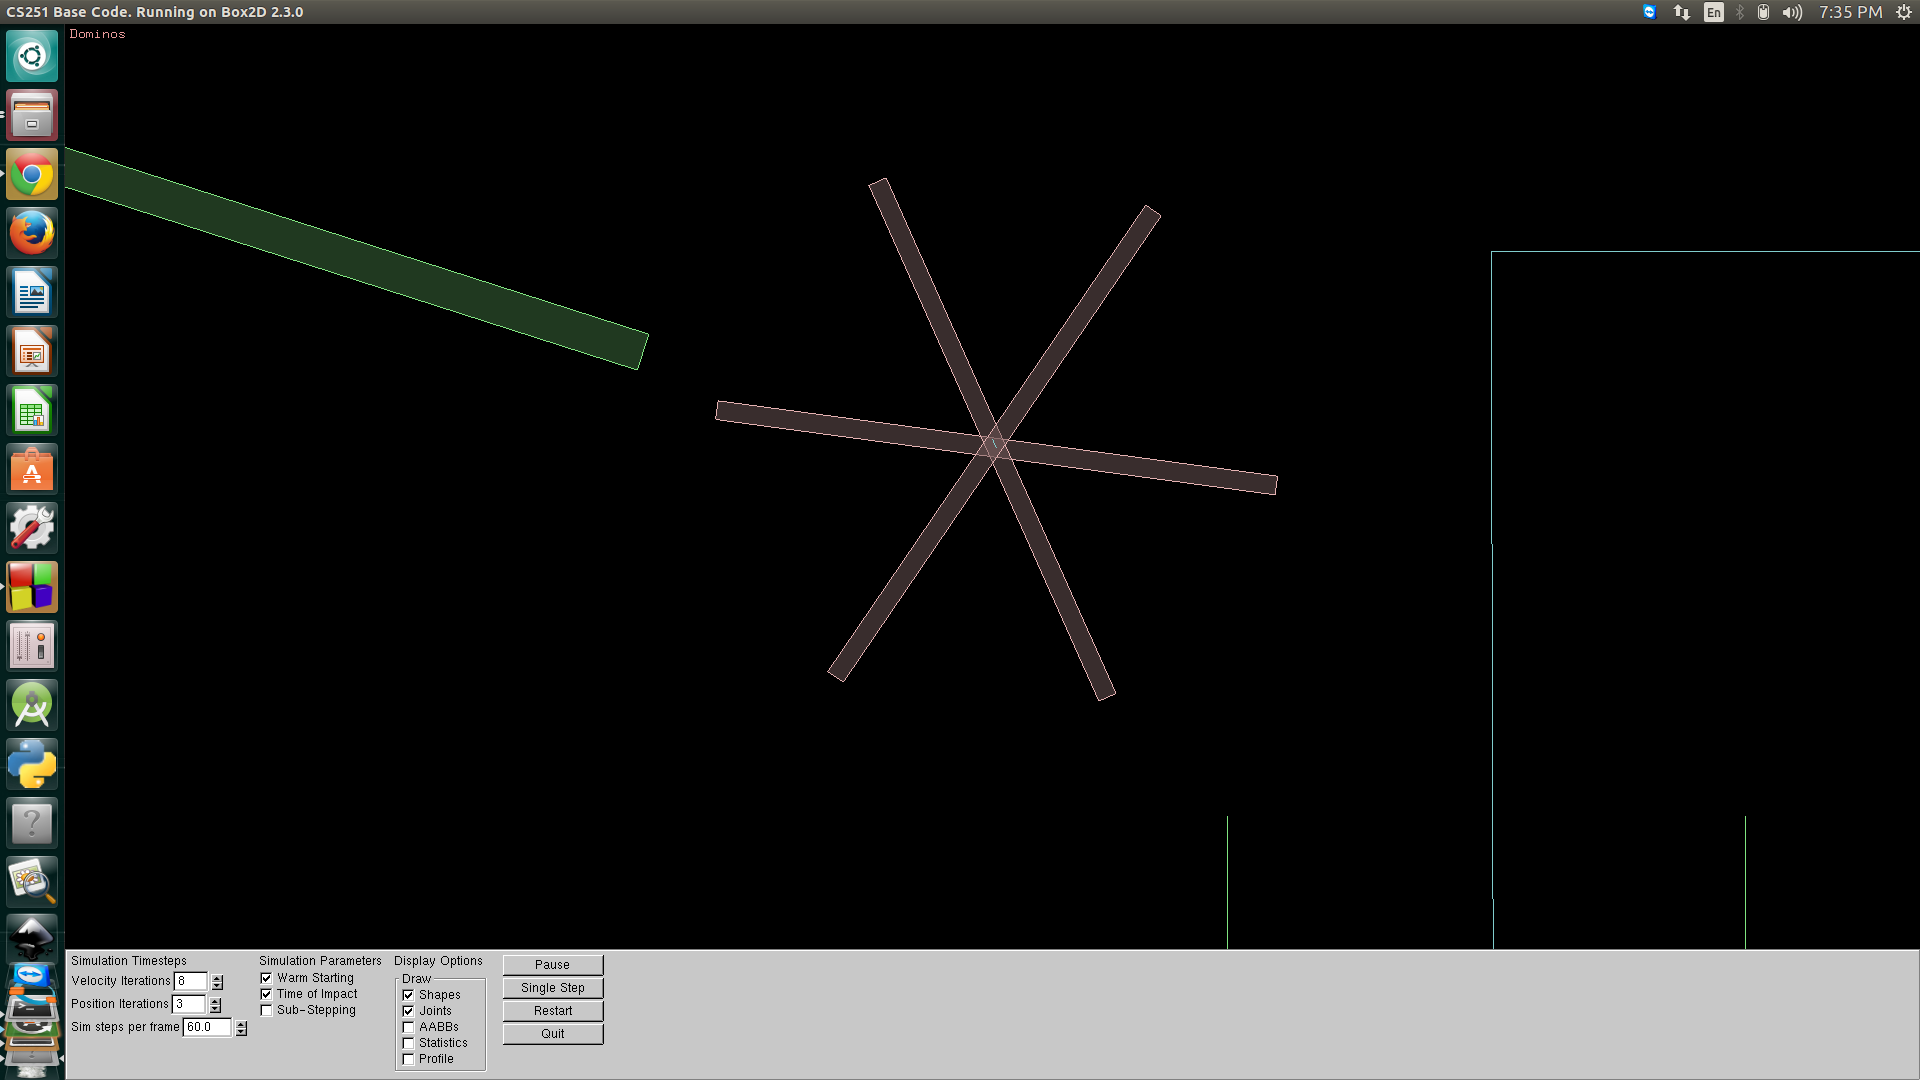
\includegraphics[scale=0.2]{project/images/rotor.png}
  \caption{\textbf{MOTOR}}
\end{figure}

\section{the second pulley}
\paragraph{
the construction is almost similar to the first pulley
Meanwhile the balls from the motor fall  into the open box of the pulley,which makes it unbalanced and hence the open box moves down and the plank on the right side moves left.
}
\begin{figure}[H]
  \centering
    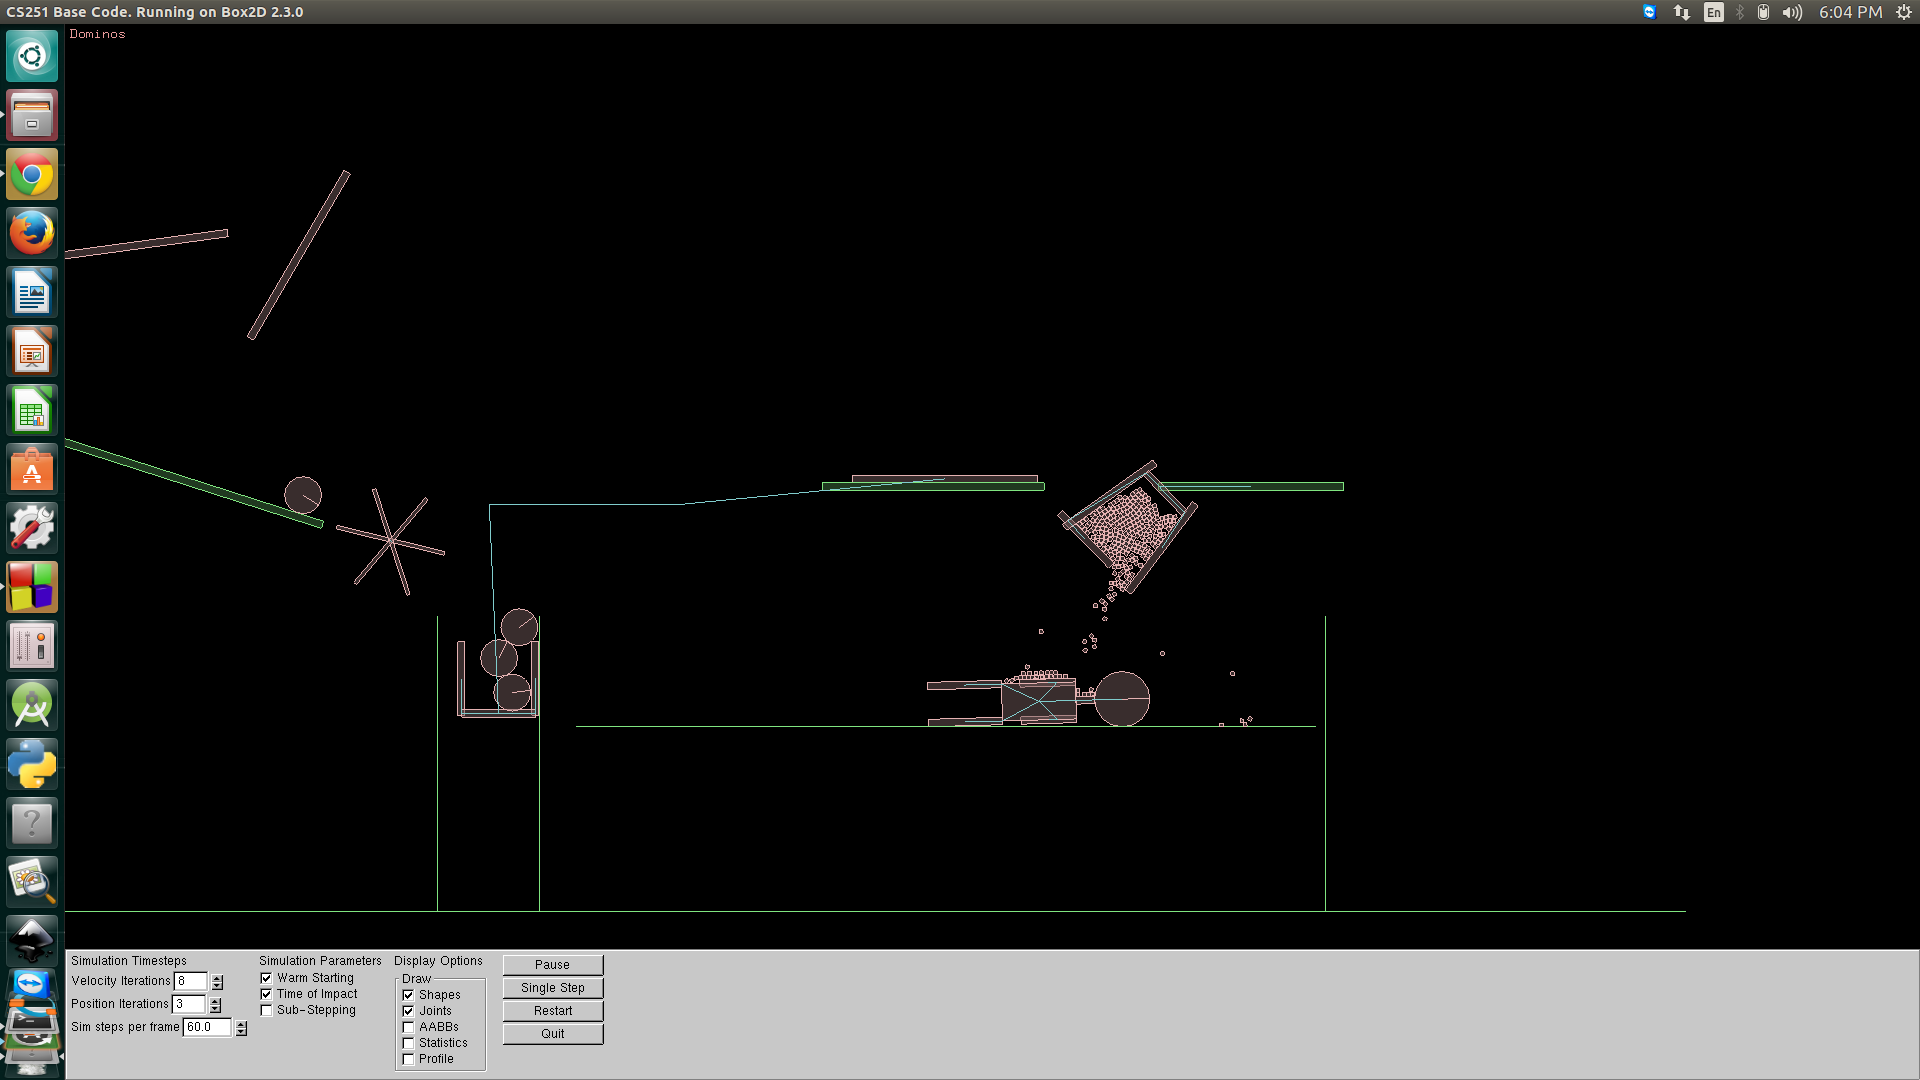
\includegraphics[scale=0.2]{project/images/bucket.png}
  \caption{\textbf{SECOND PULLEY}}
\end{figure}


\section{Bucket full of water}
\paragraph{
the construction of the bucket is similar to the oopen box.
just that the angles of the side blocks are changed.
also it has a lid which is also a block attached using a weld joint.
the water is made using small blocks of size 0.1/0.1
The bucket is attached to a static rectangular plank on the right side, with a revolute joint.
It is also supported using the plank which is connected to the pulley.
now when the pulley was disturbed the plank moves left and hence the bucket looses balance and rotates around the revolute joint.
now the water from the bucket falls down due to gravity on the face of the man and the man wakes up.
}
\begin{figure}[H]
  \centering
    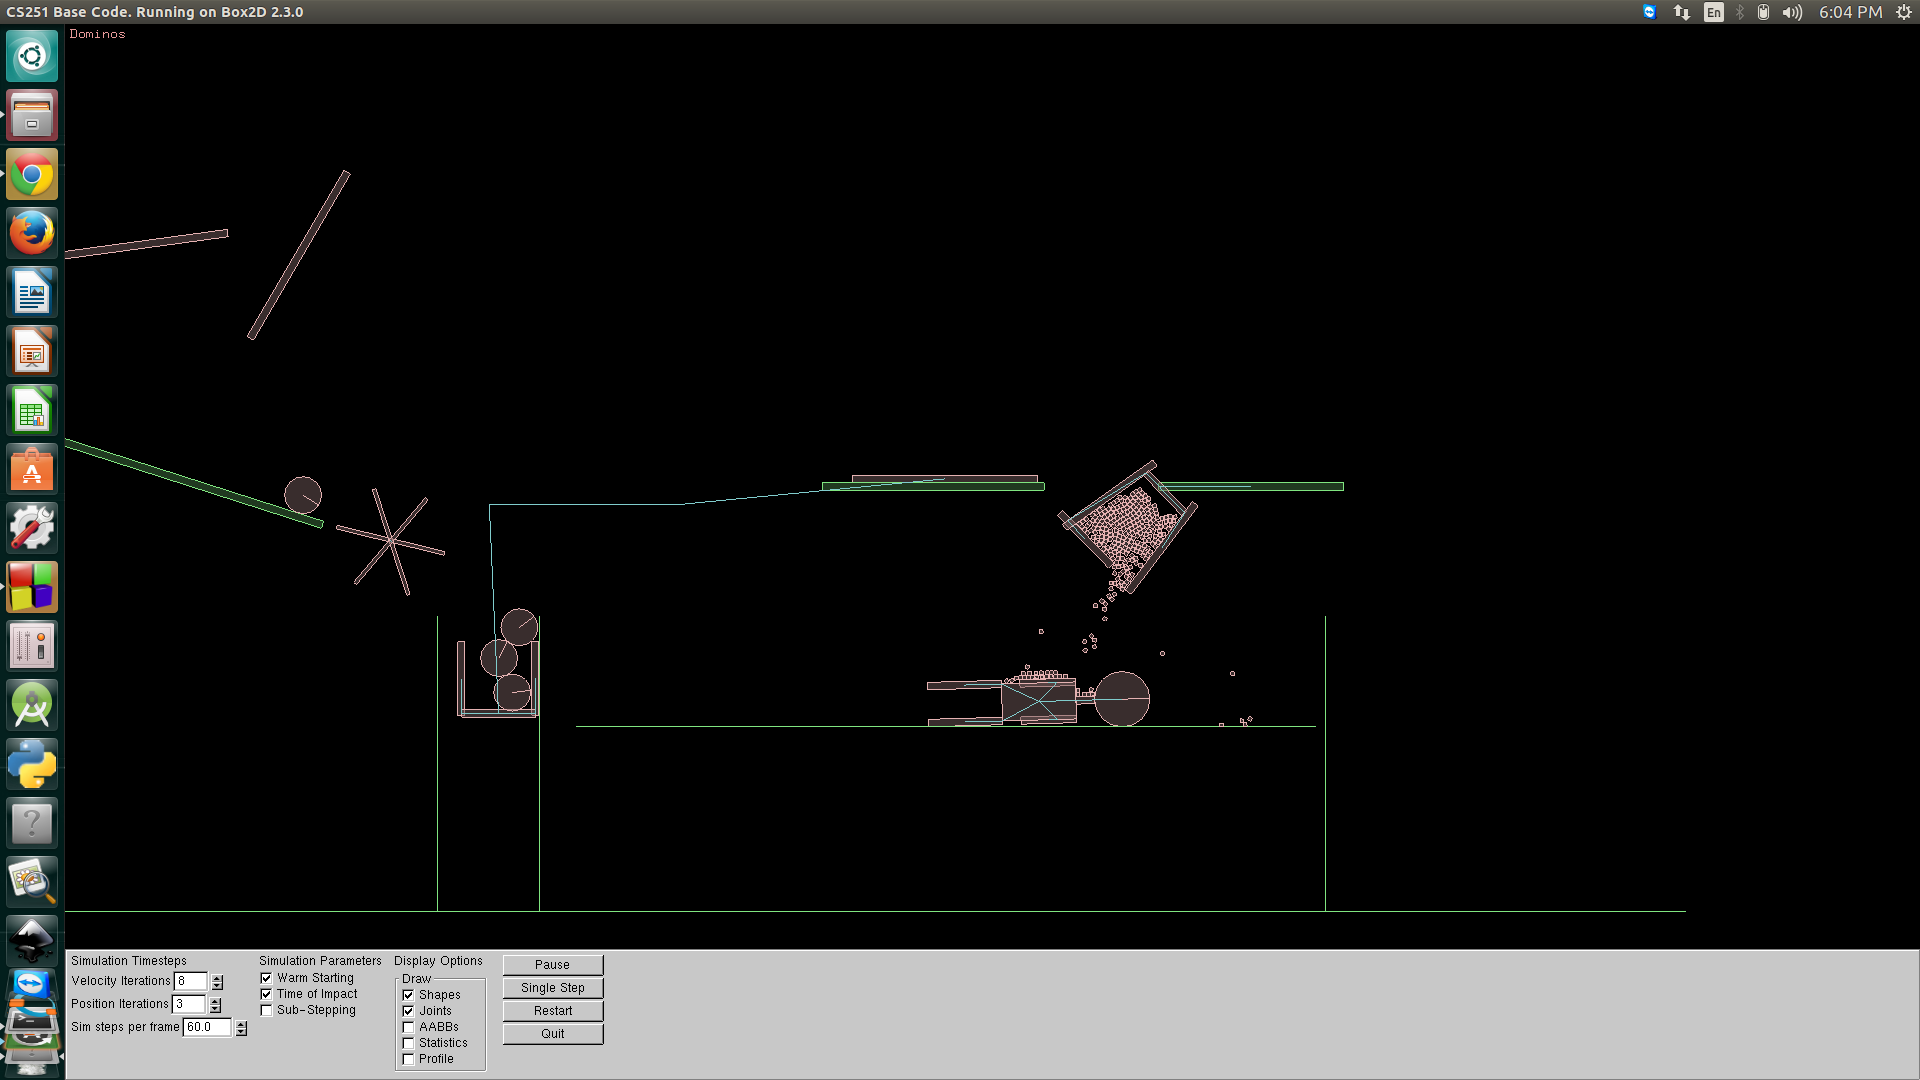
\includegraphics[scale=0.2]{project/images/bucket.png}
  \caption{\textbf{BUCKET}}
\end{figure}

